\documentclass[10pt,a4paper]{article}
\usepackage[utf8]{inputenc}
\usepackage[spanish]{babel}
\usepackage{amsmath}
\usepackage{amsfonts}
\usepackage{amssymb}
\usepackage{multicol}
\usepackage{graphicx}
\usepackage[left=2cm,right=2cm,top=2cm,bottom=2cm]{geometry}
\author{Rodrigo Francisco}
\title{Serie 1}
\begin{document}

	\begin{center}
	{\LARGE \bf Cálculo}\\
	{\large  \bf Serie 1}\\
	enero 2019
	\end{center}
\begin{multicols*}{2} 	
	\section{Dominio y Rango de una función}	
	
    
        \begin{enumerate}
            \item Dominio y rango de la función ilustrada            						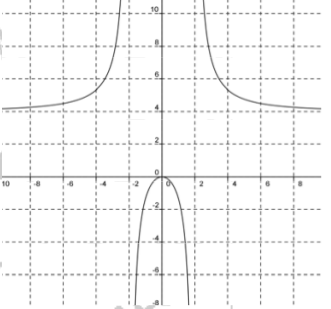
\includegraphics[width=7cm]{img/s1-35}
            \item El dominio de la función cuya gráfica se presenta a 		continuación, es:
            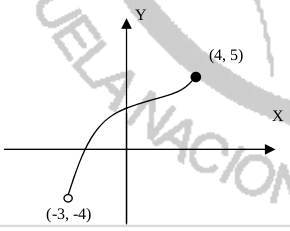
\includegraphics[width=7cm]{img/s1-38}
            \item El dominio de la función \\ $g=\{(3,2),(5,0),(7,-2),(8,7),(9,-10)\}$
            \item El dominio de la función $y=x^2$
            \item El dominio de $f(x) = \dfrac{x^2-9}{x-3}$
            \item El dominio de la función $y=\dfrac{x}{x^2-1}$
            \item El dominio de $f(x) = \dfrac{x}{x^2+x-6}$
            \item Obtener el dominio de la función $f(x) = \sqrt{2-3x}$
            \item El rango o imagen del dibujo de la función es:
            	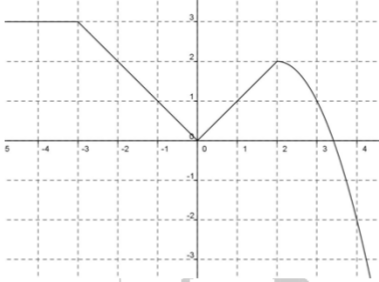
\includegraphics[width=7cm]{img/s1-87}
            \item El recorrido ó imgane de la relación $y=x^2-3$
            \item El rango de la función $xy+y=1$
            \item El rango de la función dado por $f(x) = \dfrac{2}{1-x}$
        \end{enumerate}
    
    \section{Operaciones con funciones}	
	
        \begin{enumerate}
			\item si $f(x) = \sqrt{x}$ y $g(x) = x^2+1$ entonces la operación $(f \bullet g) $ es
			\item Sean $f(x)=3x+1$, $g(x) = \dfrac{3}{x^2-x}$ con $x \neq 0,1$ y $h(x) = \sqrt[2]{3x+2}$, con $x \geq - \dfrac{2}{3}$ Calcular lo siguiente
			\begin{enumerate}
				\item La composición de $(g \circ f)(x)$
				\item La composición de $(h \circ f)(x)$
				\item La composición de $(g \circ f \circ h)(x)$
				\item La operación de $f(x)-g(x)h(x)+(g \circ f)(3)$
			\end{enumerate}
        \end{enumerate}
    
        \section{Límites}	
	
        \begin{enumerate}
			\item Indica la opción donde $\lim\limits_{x \to x_0} f(x)$ existe		
			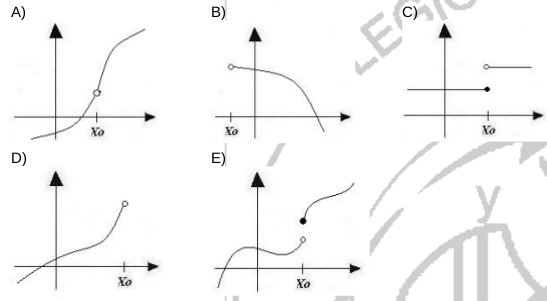
\includegraphics[width=7cm]{img/s4-6}
			\item El valor del $\lim\limits_{x \to -\frac{2}{3}} \dfrac{x^2-3x+1}{1-x}$
			\item El limite de $y = 3 sin(2x)$ cuando "x" tiende a $\dfrac{\pi}{4}$ es
        \end{enumerate}
        
        \subsection{Límites indeterminados}
        
        \begin{enumerate}
        	\item El $\lim\limits_{x \to 3} \dfrac{x^2+x-2}{x^2-9}$
        	\item Calcula el valor de $\lim\limits_{x \to 5} \dfrac{1-\frac{3}{x}}{x^2-9}$
        	\item El $\lim\limits_{x \to -3} \sqrt{\dfrac{x^2-9}{2x^2+7x+3}}$
        \end{enumerate}
        
	\section{Derivadas}
	\begin{enumerate}
		\item La derivada del siguiente polinomio $f(x) = \dfrac{1}{4}x^4+3x^3-5x^2+6x-18$
		\item La pendiente de la recta tangente a la curva $y = x^3+2x^2-x-10$ en el punto (-2,8) es:
		\item La derivada con respecto a "x" de $f(x) = 8x^2 + \dfrac{3}{x^2}$
		\item La derivada de la función $y = 2x^{\frac{1}{2}}+3x^{\frac{1}{3}}$
	\end{enumerate}
	
	\subsection{Derivada del producto y la división}
	
	\begin{enumerate}
		\item La derivada de $y = \dfrac{2}{2x-1}$
		\item La derivada de $(2x+1)(4x^2-2)$
		\item La derivada de $\left(\dfrac{x+1}{x+2}\right)(2x-5)$ es
	\end{enumerate}
	
	
	\subsection{Regla de la cadena}
	\begin{enumerate}
		\item La derivada de la función $f(x) = (8x-4)^5$
		\item La derivada de la función $f(x) = \dfrac{(6x+1)^4}{(1-x)^4}$
		\item La derivada de $f(x) = [3+(5x-1)^10]^10$
		\item Si $f(x) = \sqrt{1+ \sqrt{x}}$ entonces $f'(1)$
	\end{enumerate}
	
	\subsection{Derivada implícita}
	\begin{enumerate}
		\item El resultado de derivar $15x = 15y+5y^3 + 3y^5$
		\item La deriviada implícita de $\dfrac{1}{x^2}+\dfrac{1}{y^2}= 2$ es:
	\end{enumerate}
	
	\subsection{Derivada de orden superior}
	
	\begin{enumerate}
		\item La segunda derivada de $y = \dfrac{16}{x+4}$
		\item La segunda derivada de $f(x) = x^2-3x+5$
	\end{enumerate}
	
	 \section{Máximos y mínimos de una función}
		\begin{enumerate}
		\item Identificar los puntos críticos de la función y decir si son máximos o mínimos de $y = x^2-6x^2+12x-12$
		\item El máximo o mínimo de $f(x) = x^2+\dfrac{432}{x}$
		\item Los puntos máximos y mínimos de $f(x) = 2x^3-3x^2-12x+2$
	\end{enumerate}
	
\end{multicols*}
\end{document}